% ==================================================================
%  HSE Homework Assignment — single-file template (fixed)
%  Compile: pdflatex assignment.tex   (twice)
% ==================================================================
\documentclass[11pt,a4paper]{article}
\usepackage{fix-cm} 
% ---------- Encoding & language (English only) ----------
\usepackage[T1]{fontenc}
\usepackage[utf8]{inputenc}
\usepackage[english]{babel}

% ---------- Geometry ----------
\usepackage[
  left=30mm, right=25mm,
  top=25mm, bottom=25mm,
  headsep=12pt, footskip=15pt
]{geometry}

% ---------- Math (must come before newtxmath) ----------
\usepackage{amsmath}
\usepackage{bm}

% ---------- Fonts (Times-like; supplies all AMS symbols) ----------
\usepackage{newtxtext,newtxmath}

% ---------- Spacing ----------
\usepackage{setspace}
\setstretch{1.15}

% ---------- Tables & figures ----------
\usepackage{booktabs,array,tabularx,multirow}
\usepackage{graphicx}
\usepackage{float}
\usepackage{caption}
\captionsetup{font=small,labelfont=bf,skip=4pt}

% ---------- Lists ----------
\usepackage{enumitem}
\setlist{itemsep=2pt,topsep=3pt,parsep=0pt,leftmargin=*}

% ---------- Typography ----------
\usepackage{microtype}

% ---------- Citations (Harvard author–year) ----------
\usepackage[authoryear,round]{natbib}

% ---------- Hyperref (load last) ----------
\usepackage[hidelinks]{hyperref}
\hypersetup{colorlinks=true,linkcolor=black,citecolor=black,urlcolor=blue}

% ---------- Paragraph style ----------
\setlength{\parindent}{1.5em}
\setlength{\parskip}{0.3ex plus 0.1ex minus 0.1ex}

% ---------- Headers / footers ----------
\usepackage{fancyhdr}
\pagestyle{fancy}
\fancyhf{}
\fancyfoot[C]{\small\thepage}
\renewcommand{\headrulewidth}{0pt}
\fancypagestyle{plain}{%
  \fancyhf{}\fancyfoot[C]{\small\thepage}%
  \renewcommand{\headrulewidth}{0pt}}

% ---------- Metadata (edit per assignment) ----------
\usepackage{pgfkeys}
\newcommand{\HSEnumber}{}\newcommand{\HSEtitle}{}
\newcommand{\HSEcourse}{}\newcommand{\HSEprogramme}{Master's Programme}
\newcommand{\HSEstudent}{}\newcommand{\HSEgroup}{}
\newcommand{\HSEsupervisor}{}\newcommand{\HSEdate}{}
\pgfkeys{
  /hse/.is family, /hse,
  number/.store in     = \HSEnumber,
  title/.store in      = \HSEtitle,
  course/.store in     = \HSEcourse,
  programme/.store in  = \HSEprogramme,
  student/.store in    = \HSEstudent,
  group/.store in      = \HSEgroup,
  supervisor/.store in = \HSEsupervisor,
  date/.store in       = \HSEdate,
}
\newcommand{\HSESetup}[1]{\pgfkeys{/hse,#1}}

% ---------- Title page + running header ----------
\renewcommand{\maketitle}{%
  \begin{titlepage}%
    \thispagestyle{empty}\centering
    \vspace*{1.2cm}
    {\Large\scshape National Research University\\[0.2em]
     Higher School of Economics\par}
    \vspace{0.4cm}{\normalsize Faculty of Computer Science\par}
    \vspace{2.5cm}
    \rule{\linewidth}{0.5pt}\\[0.7cm]
    {\Huge\bfseries Spotify Tracks Analysis: Regression, Correlation, and PCA/SVD~\HSEnumber\par}
    \vspace{0.5cm}
    {\LARGE\itshape \HSEtitle\par}
    \vspace{0.7cm}\rule{\linewidth}{0.5pt}
    \vfill
    {\large\renewcommand{\arraystretch}{1.25}%
     \begin{tabular}{@{}rl@{}}
       \textbf{Course:}     & \HSEcourse \\[0.3em]
       \textbf{Programme:}  & \HSEprogramme \\[0.3em]
       \textbf{Student:}    & \HSEstudent \\[0.3em]
       \textbf{Group:}      & \HSEgroup \\[0.3em]
       \textbf{Supervisor:} & \HSEsupervisor \\
     \end{tabular}\par}
    \vfill{\large \HSEdate\par}\vspace{0.5cm}
  \end{titlepage}%
  \pagenumbering{arabic}%
  \pagestyle{fancy}\fancyhf{}%
  \fancyhead[L]{\small\itshape \HSEcourse}%
  \fancyhead[R]{\small\itshape Assignment~\HSEnumber}%
  \fancyfoot[C]{\small\thepage}%
  \renewcommand{\headrulewidth}{0.4pt}%
  \hypersetup{pdftitle={Assignment \HSEnumber: \HSEtitle},
              pdfauthor={\HSEstudent}}%
}

% ==================================================================
\begin{document}
% ==================================================================

\HSESetup{
  number     = {1 and 2},
  title      = {Regression, Correlation, and PCA/SVD},
  course     = {Basics of Data Analysis},
  student    = {S M Gazzali Arafat Nishan},
  group      = {Data Science},
  supervisor = {professor Boris Mirkin},
  date       = {Moscow -- 2026},
}

\maketitle
\tableofcontents
\newpage

% ==================================================================
\section{Introduction}

This report presents the solutions of Homework Assignments~A1 and A2 for the course
\textit{Basics of Data Analysis}. The analysis follows the approximation
(least-squares) perspective of two-dimensional linear regression and the
correlation framework introduced in Lecture~2 \citep{lecture}, building on
the classical treatment of \citet{galton,pearson}.

The original Spotify Tracks dataset \citep{spotify} contains approximately
114\,000 observations and 21 variables spanning 114 genres. On the advice of
the supervisor the study was restricted to a single homogeneous
genre---\textbf{pop}---yielding a clean subset of $n=1\,000$ complete
observations. The selected feature pair is
\begin{itemize}
  \item predictor $X$: \texttt{energy} (perceptual intensity, scaled on $[0,1]$);
  \item target $Y$: \texttt{loudness} (overall loudness in dB).
\end{itemize}

All calculations use the ordinary-least-squares (OLS) closed form; a random
80/20 train/test split (seed~42) supports the machine-learning evaluation view.

% ==================================================================
\section{Feature selection}

Among the numeric audio features the pair \texttt{energy}--\texttt{loudness}
exhibits a clear positive linear tendency inside the pop subset and is readily
interpretable: energetic tracks tend to be mastered at higher loudness levels.
The pair therefore satisfies the lecture requirement of a ``more or less
linear-like'' scatter-plot and was retained.

% ==================================================================
\section{Scatter-plot and suitability for linear regression}

\begin{figure}[H]
  \centering
  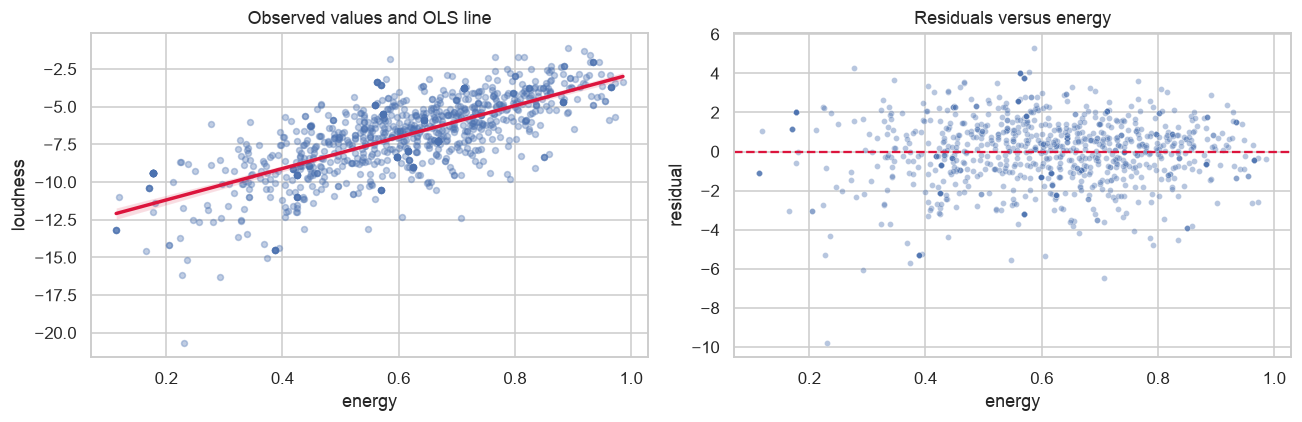
\includegraphics[width=0.95\textwidth]{pop_energy_loudness_analysis.png}
  \caption{Energy versus loudness for the pop genre ($n=1\,000$):
    fitted OLS line (left) and residual plot (right).}
  \label{fig:scatter}
\end{figure}

The cloud of points rises from left to right, confirming a positive association.
A straight line captures the dominant trend, yet a residual spread of several
decibels remains visible. A linear model is therefore a reasonable
\emph{baseline} (approximation perspective), but energy alone cannot determine
loudness with high precision; production style, compression and instrumentation
still play important roles.

% ==================================================================
\section{Linear regression and interpretation of the slope}

\subsection{Ordinary-least-squares formulae}

The model is written
\begin{equation}
  \hat{y}_i = \beta_0 + \beta_1 x_i .
\end{equation}
The estimators that minimise the residual sum of squares $\sum e_i^2$ are
\begin{align}
  \beta_1 &= \frac{S_{xy}}{S_{xx}}, \qquad
  S_{xx} = \sum_{i=1}^n (x_i-\bar{x})^2, \qquad
  S_{xy} = \sum_{i=1}^n (x_i-\bar{x})(y_i-\bar{y}), \\[0.3em]
  \beta_0 &= \bar{y} - \beta_1 \bar{x}.
\end{align}

\subsection{Numerical values on the pop subset}

\begin{align*}
  \bar{x} &= 0.606437, & \bar{y} &= -6.953969, \\
  S_{xx}  &= 31.553180, & S_{xy} &= 328.963185.
\end{align*}
Hence
\begin{align*}
  \beta_1 &= \frac{328.963185}{31.553180} = 10.425675, \\
  \beta_0 &= -6.953969 - 10.425675 \times 0.606437 = -13.276484.
\end{align*}
The fitted equation is therefore
\begin{equation}
  \boxed{\mathrm{loudness} = -13.2765 + 10.4257 \times \mathrm{energy}.}
\end{equation}

\subsection{Meaning of the slope}

The slope $\beta_1 = 10.4257$ is the expected change in loudness (dB) when
energy increases by one full unit. Because energy is scaled on the unit
interval a more practical statement is
\begin{equation}
  \Delta\mathrm{energy}=0.1 \quad\Rightarrow\quad
  \Delta\mathrm{loudness}\approx 1.043\,\mathrm{dB}.
\end{equation}
This is an observed association, not a causal claim.

% ==================================================================
\section{Correlation coefficient and determinacy coefficient}

\subsection{Pearson correlation \texorpdfstring{$\rho$}{rho}}

\begin{equation}
  \rho = \frac{\mathrm{Cov}(X,Y)}{s_X\,s_Y}.
\end{equation}
On the pop data
\begin{align*}
  \mathrm{Cov}(X,Y) &= 0.328963, \\
  s_X &= 0.177632, \qquad s_Y = 2.561336,
\end{align*}
yielding
\begin{equation}
  \rho = \frac{0.328963}{0.177632 \times 2.561336} = 0.7230 .
\end{equation}
The value indicates a moderately strong positive linear association.

\subsection{Determinacy coefficient \texorpdfstring{$\rho^2$}{rho-squared}}

\begin{equation}
  \rho^2 = r^2 = (0.7230)^2 = 0.5228 \quad (52.28\,\%).
\end{equation}
Equivalently, from the sum-of-squares decomposition
\begin{align*}
  SS_{\mathrm{tot}} &= 6560.441, \\
  SS_{\mathrm{res}} &= 3130.777, \\
  SS_{\mathrm{reg}} &= 3429.663,
\end{align*}
\begin{equation}
  \rho^2 = 1 - \frac{SS_{\mathrm{res}}}{SS_{\mathrm{tot}}} = 0.5228 .
\end{equation}

\textbf{Interpretation (Lecture~2).} Approximately 52\,\% of the observed
variation in loudness is accounted for by the linear relationship with energy;
the remaining 48\,\% is unexplained. A moderate-to-high determinacy does
\emph{not} automatically guarantee high precision of individual
predictions---the residual standard deviation remains about 1.77\,dB.

% ==================================================================
\section{Predictions for selected predictor values}

Substituting four convenient energy levels into the fitted equation produces
the conditional means shown in Table~\ref{tab:pred}.

\begin{table}[H]
\centering
\caption{Predicted loudness for four energy values.}
\label{tab:pred}
\begin{tabular}{cccc}
\toprule
Energy $x$ & Calculation & Predicted loudness (dB) \\
\midrule
0.2 & $-13.2765 + 10.4257 \times 0.2$ & $-11.191$ \\
0.4 & $-13.2765 + 10.4257 \times 0.4$ & $-9.106$  \\
0.6 & $-13.2765 + 10.4257 \times 0.6$ & $-7.021$  \\
0.8 & $-13.2765 + 10.4257 \times 0.8$ & $-4.936$  \\
\bottomrule
\end{tabular}
\end{table}

These figures are average model estimates. Because the residual standard
deviation is approximately 1.77\,dB, an individual track with the same energy
can easily deviate by $\pm2$--$3$\,dB. The predictions should therefore be
regarded as tendencies rather than exact forecasts.

% ==================================================================
\section{Mean relative absolute error: DA and ML views}

Lecture~2 distinguishes two relative-error definitions:
\begin{align}
  \Delta_{\mathrm{DA}}(i) &= \frac{|y_i-\hat{y}_i|}{|y_i|}
    && \text{(data-analysis / descriptive view)}, \\[0.4em]
  \Delta_{\mathrm{ML}}(i) &= \frac{|y_i-\hat{y}_i|}{|\hat{y}_i|}
    && \text{(machine-learning view)}.
\end{align}

\subsection{Full-sample (DA) results}

\begin{align*}
  \mathrm{MAE}   &= 1.376\,\mathrm{dB}, \\
  \mathrm{RMSE}  &= 1.769\,\mathrm{dB}, \\
  \mathrm{MRAE}_{\mathrm{DA}} &= 23.13\,\%, \\
  \mathrm{MRAE}_{\mathrm{ML}} &= 20.44\,\%.
\end{align*}

\subsection{Train/test (ML) results}

A random 80/20 partition (seed~42) yields 800 training and 200 held-out test
tracks. Re-estimating on the training data alone gives
\[
  \beta_1^{\mathrm{train}} = 10.5213, \qquad
  \beta_0^{\mathrm{train}} = -13.3293.
\]
On the unseen test observations:
\begin{align*}
  \mathrm{Test\,MAE} &= 1.438\,\mathrm{dB}, \\
  \mathrm{Test\,MRAE}_{\mathrm{DA}} &= 23.53\,\%, \\
  \mathrm{Test\,MRAE}_{\mathrm{ML}} &= 21.34\,\%.
\end{align*}
The held-out figures remain close to the full-sample figures, indicating that
the linear relationship generalises well inside the homogeneous pop genre.

% ==================================================================
\section{Comparison of errors and the determinacy coefficient}

\begin{table}[H]
\centering
\caption{Summary of determinacy and relative-error metrics.}
\label{tab:compare}
\begin{tabular}{lcc}
\toprule
Quantity & Value & Comment \\
\midrule
Determinacy $\rho^2$ (all data) & 0.5228 & 52\,\% of variance explained \\
Train $\rho^2$                 & 0.5259 & almost identical \\
Test $\rho^2$                  & 0.5101 & only a tiny drop \\
MRAE$_{\mathrm{DA}}$ (all)     & 23.13\,\% & lecture DA definition \\
MRAE$_{\mathrm{ML}}$ (all)     & 20.44\,\% & lecture ML definition \\
Test MRAE$_{\mathrm{DA}}$ / MRAE$_{\mathrm{ML}}$ & 23.53\,\% / 21.34\,\% & held-out performance \\
\bottomrule
\end{tabular}
\end{table}

\paragraph{Key observations aligned with the lecture.}
\begin{enumerate}
  \item The test $\rho^2$ (0.510) is only 0.016 lower than the training
        $\rho^2$ (0.526); the linear pattern is stable and no serious
        over-fitting is observed.
  \item An $\rho^2$ of approximately 0.52 leaves a residual standard deviation
        of roughly 1.8\,dB; individual predictions remain imprecise.
  \item The DA and ML relative errors differ because the denominator changes
        ($|y|$ versus $|\hat{y}|$); both stay in the 20--24\,\% range.
  \item Restricting the analysis to a single genre avoids the
        Simpson-paradox situation illustrated in the lecture for the full
        multi-taxon Iris data.
\end{enumerate}

% ==================================================================
\section{Residual diagnostic}

The residual-versus-energy plot (right panel of Figure~\ref{fig:scatter}) is
roughly centred on zero and shows no strong systematic curvature, supporting
the linear specification. The vertical spread nevertheless remains substantial
(some residuals exceed $\pm5$\,dB), confirming that energy is only one of the
factors related to loudness. A few low-energy tracks produce large negative
residuals and would merit closer inspection before the model is used for any
high-stakes decision.

% ==================================================================
\section{Reproducibility notes}

\begin{itemize}
  \item OLS estimates obtained analytically (identical to
        \texttt{sklearn.linear\_model.LinearRegression}).
  \item Train/test split: 20\,\% held out, random permutation seeded with~42.
  \item Pearson $\rho$ and $\rho^2$ computed on the full pop subset of
        $1\,000$ complete cases; no missing values for the two selected features.
  \item Relative-error definitions follow Lecture~2
        (DA: division by $|y|$; ML: division by $|\hat{y}|$).
\end{itemize}

% ==================================================================
\section{Conclusion}

A linear regression of loudness on energy was fitted to the homogeneous pop
subset of the Spotify Tracks dataset. The resulting model
\[
  \mathrm{loudness} = -13.2765 + 10.4257 \times \mathrm{energy}
\]
explains 52.3\,\% of the variance ($\rho = 0.723$). Absolute and relative
errors stay moderate (MAE $\approx 1.4$\,dB, MRAE $\approx 23\,\%$), and the
train/test gap is negligible. The analysis illustrates the lecture's central
messages: a respectable determinacy coefficient does not guarantee high
individual precision, the DA and ML relative-error views differ, and restricting
attention to a single genre removes the confounding that can produce
Simpson-type paradoxes.

% ==================================================================
\section{Assignment A2: PCA/SVD, visualization, and hidden ranking factor}

\subsection{Feature subset, preprocessing, and group}

Following Lecture~3 \citep{lecture3}, PCA is treated as a least-squares low-rank approximation
of a preprocessed data matrix. We selected four continuous audio features that
jointly describe musical intensity and affect: \texttt{energy},
\texttt{loudness}, \texttt{danceability}, and \texttt{valence}. Loudness is
measured in dB, while the other features are on $[0,1]$, so preprocessing is
necessary before comparing their contributions. We retained one row per
\texttt{track\_id}, removed rows missing any selected feature or the group
label, and obtained $n=89\,741$ tracks. Explicit tracks (7,705 observations)
were designated in advance as the group highlighted in both visualizations.

For range normalization, each feature was transformed as
\[
 x'_{iv}=\frac{x_{iv}-\min_i x_{iv}}{\max_i x_{iv}-\min_i x_{iv}}-\frac12,
\]
so the observed range is centered at zero. For z-scoring, we used
$z_{iv}=(x_{iv}-\bar{x}_v)/s_v$, with sample standard deviation $s_v$.
These choices change the PCA because the method depends on preprocessing.

\subsection{SVD, scatter, and component contributions}

For each transformed matrix $X$, the singular value decomposition is
$X=U\Sigma V^T$. Its total data scatter is
$\|X\|_F^2=\sum_k\sigma_k^2$, and component $k$ contributes
$\sigma_k^2$, or $100\sigma_k^2/\|X\|_F^2$ percent. The first two
contributions are:
\begin{center}
\begin{tabular}{lrrrrrr}
\toprule
Normalization & Scatter & $\sigma_1$ & PC1 contribution & $\sigma_2$ & PC2 contribution & First two total \\
\midrule
Range centered & 24,057.89 & 113.84 & 53.87\% & 82.26 & 28.13\% & 81.99\% \\
Z-score & 358,964.00 & 436.91 & 53.18\% & 319.08 & 28.36\% & 81.54\% \\
\bottomrule
\end{tabular}
\end{center}

For the range-normalized case, the first component contributes 53.87\% and
the second 28.13\% (81.99\% together). The leading range loadings are
energy (0.687) and loudness (0.637) on PC1; valence (0.906) dominates PC2.
Under z-scoring, PC1 has positive loadings on all four features, with energy
(0.544) and loudness (0.580) largest. PC2 contrasts danceability (0.608) and
valence (0.512) against loudness and energy after the sign convention shown
in the code. The sign of an entire component is arbitrary; relative signs
carry the interpretation.

The first two PC coordinates retain 81.99\% of range-normalized scatter and
81.54\% of z-scored scatter. The highlighted explicit tracks have a slightly
higher mean PC1 score than other tracks in both visualizations (range:
0.370 versus 0.262; z-score: 0.539 versus $-0.051$). The PC2 means are nearly
the same (range: $-0.100$ versus $-0.098$; z-score: 0.058 versus $-0.005$),
so there is no clear group separation along PC2. These are descriptive
positions, not evidence that explicit content causes audio-feature changes.

\subsection{Conventional PCA comparison}

The conventional calculation forms the correlation matrix
$B=Y^TY/(n-1)$ from the z-scored matrix $Y$ and diagonalizes it. The resulting
variance shares are 53.18\%, 28.36\%, 12.76\%, and 5.69\%, matching the
z-score SVD contributions. Loadings and scores agree with the model-based
z-score solution up to sign and the conventional score scaling. Since the
features have different original units, z-scoring is the more balanced
choice here: it gives each feature unit variance and is exactly the input
required by conventional correlation-matrix PCA. Range normalization instead
makes the observed spans equally important. Neither preprocessing is
universally best; the choice expresses what differences should count.

\subsection{Hidden ranking factor}

Each selected feature was converted to a percentile rank on $[0,100]$. We
then took the first right singular vector of this ranked matrix, oriented it
to have positive weights, and normalized its weights to sum to one. The
resulting weights are energy 0.252, loudness 0.254, danceability 0.245, and
valence 0.250. The hidden score is their weighted sum of feature ranks,
rescaled so the maximum observed score is 100. In this sample the score has
median 53.74 and interquartile range 37.97--66.66; the explicit group mean is
59.12 versus 50.69 for other tracks. This is a sample-relative summary of
these four features, not a measure of quality. The calibration anchor (the
maximum observed composite equals 100) is stated because a component score's
scale is otherwise arbitrary.

\paragraph{Reproducibility and interpretation.}
All A2 calculations use the Python 3.14.7 environment recorded in the
notebook, NumPy SVD, and the exact feature transformations defined above.
The executable code and task-by-task explanations are in the accompanying
\texttt{bda.ipynb}. Singular-vector signs may reverse across software runs
without changing the PCA solution.

% ==================================================================
\section*{References}
\addcontentsline{toc}{section}{References}

\begin{thebibliography}{9}

\bibitem[Galton(1886)]{galton}
Galton, F. (1886).
\newblock Regression towards mediocrity in hereditary stature.
\newblock \textit{Journal of the Anthropological Institute}, 15, 246--263.

\bibitem[Pearson(1895)]{pearson}
Pearson, K. (1895).
\newblock Notes on regression and inheritance in the case of two parents.
\newblock \textit{Proceedings of the Royal Society of London}, 58, 240--242.

\bibitem[Kaggle(2020--2024)]{spotify}
Kaggle (2020--2024).
\newblock \textit{Spotify Tracks Dataset (114k songs)}.
\newblock \url{https://www.kaggle.com/datasets/maharshipandya/spotify-tracks-dataset}

\bibitem[Mirkin(2026)]{lecture}
Mirkin, B. (2026).
\newblock \textit{Basics of Data Analysis. Lecture 2: 2D Regression and
  Correlation Coefficient}.
\newblock HSE University, lecture notes.

\bibitem[Mirkin(2026b)]{lecture3}
Mirkin, B. (2026).
\newblock \textit{Basics of Data Analysis. Lecture 3: Principal Component
Analysis and SVD}.
\newblock HSE University, lecture notes.

\end{thebibliography}

\end{document}